% 
% Annual Cognitive Science Conference
% Sample LaTeX Paper -- Proceedings Format
% \


% to do
% -- consistent names of conditions: listener uncertainty in common ground vs. not
% -----

\documentclass[10pt,letterpaper]{article}

\usepackage{cogsci}
\usepackage{pslatex}
\usepackage{apacite}
\usepackage{url}
\usepackage{graphicx}
\usepackage{caption}
\usepackage{subcaption}
\usepackage{listings}
\usepackage{color}
\usepackage{textcomp}
\usepackage{amsmath}
\usepackage{amssymb}
\usepackage{wrapfig}
\usepackage{lipsum}
\usepackage{epigraph}

\graphicspath{{figures/}}

\def\signed #1{{\leavevmode\unskip\nobreak\hfil\penalty50\hskip2em
  \hbox{}\nobreak\hfil(#1)%
  \parfillskip=0pt \finalhyphendemerits=0 \endgraf}}

\newsavebox\mybox
\newenvironment{aquote}[1]
  {\savebox\mybox{#1}\begin{quote}}
  {\signed{\usebox\mybox}\end{quote}}

 \newcommand{\denote}[1]{\mbox{ $[\![ #1 ]\!]$}}

\definecolor{Red}{RGB}{255,0,0}
\newcommand{\red}[1]{\textcolor{Red}{#1}}  

\definecolor{Blue}{RGB}{0,0,255}
\newcommand{\blue}[1]{\textcolor{Blue}{#1}}  
\definecolor{Green}{RGB}{10,200,100}
\newcommand{\ndg}[1]{\textcolor{Green}{[ndg: #1]}}  
\newcommand{\mht}[1]{\textcolor{Blue}{[mht: #1]}}  

\title{It goes without saying: The pragmatics of uninformative utterances}

\author{ {\large \bf Michael Henry Tessler*}, {\large \bf Eleanor K. Chestnut*},
{\large \bf Ellen M. Markman}, and {\large \bf Noah D. Goodman}  \\
\{mtessler, eleanor.chestnut, markman, ngoodman\} @stanford.edu \\ 
  Department of Psychology, Stanford University \\
  *Authors contributed equally to this work.}

\begin{document}

\maketitle


\begin{abstract}
\ndg{abstract is too technical. start with the puzzle of how asserting a proposition can sometimes decrease its plausibility. the use of common ground here is kind of hard to follow.}
Successful communication requires a mutually understood set of beliefs between speaker and listener.
When common ground is not shared, a listener can use a speaker's utterance in conjunction with conversational principles to infer what was assumed by the speaker.
Previous work has shown that this inference can have surprising ramifications, including decreasing the belief in the proposition that was asserted by the speaker 
(e.g. upon hearing, ``John paid the cashier!'', listeners infer that John does not typically pay for his groceries).
% i just think we need an example somewhere in here
Here, we formalize inferences about common ground using the case when a speaker's utterance refers to something that should already be in common ground.
The formal pragmatics model makes clear that this kind of utterance will backfire (i.e. imply that the opposite is typically true) when the interlocutors do not share common ground, but not when they do.
% the last sentence is a little hard to read because of many "not"s... but we can worry about that later.

%Language is interpreted in context with respect to some common ground between speaker and listener.
%Common ground can make certain utterances uninformative (e.g. stating something obvious), but is plausibly revised in the face of uninformative utterances.
%In Expt.~1, we verify this prediction using a paradigm that makes the 


\textbf{Keywords:} 
pragmatics; language; common ground; Bayesian model

\end{abstract}


%% This quote is very intuitive, though perhaps somewhat bleak for starting a paper...

%\begin{quotation}
%\small
%The day I knew incontrovertibly that my mother had some form of dementia was when my father handed me a birthday gift saying, ``Your mother picked this out all by herself.''
%Since my mother had always picked out birthday gifts, his commenting on it made me realize he had helped her.
%
%-- Carol J. Adams (``Jane Austen's Guide to Alzheimer's.'' \emph{New York Times})
%\end{quotation}

%In one of the most infamous moments in U.S. presidential history, Richard Nixon declared to the press corps, "I am not a crook"€ (CITE).  On the surface, this claim argues for Nixon's innocence, as it literally states that he is not a crook.  As several researchers have shown, however, this statement contains a number of pragmatic implications that actually counter its literal, semantic meaning (CITE).  Nixon'€™s claim, for instance, presupposes that others believed that he was a crook; otherwise, it would not have been an informative statement to make, since most people presumably are not crooks (Grice, 1975).  Thus, if a listener is not aware of the Watergate scandal, or if they have no reason to question Nixon's moral status, they might actually learn from this claim that Nixon was likely corrupt in some way.

In one of the most infamous moments in U.S. presidential history, Richard Nixon declared to the press corps, ``I am not a crook" (CITE).  On the surface, this claim argues for Nixon's innocence, as it literally states that he is not a crook.  As several researchers have shown, however, this statement contains a number of pragmatic implications that actually counter its literal, semantic meaning (CITE).  Nixon's claim, for instance, presupposes that others believed that he \emph{was} a crook; otherwise, it would not have been an informative statement to make, since most people presumably are not crooks (Grice, 1975).  Thus, if a listener (e.g., a student in a history class) is not aware of the Watergate scandal, or if they have no reason to question Nixon's moral status, they might actually \emph{learn} from this claim that Nixon was likely corrupt in some way.



	
%A few studies, however, provide preliminary evidence that utterances that are redundant with a listener'€™s preexisting beliefs do cause listeners to search for ways to make those utterances informative \cite{Yandell1979, Wegner1981, Gruenfeld1992, Kravtchenko2015}.  This process ultimately undermines the utterances' literal meanings.  

%%\citeA{Wegner1981}, for example, demonstrated that newspaper headlines such as "€Å%“Bob Talbert is not linked to the Mafia" [CHECK] cause adults to have a more negative impression of Bob than they would otherwise, despite not explicitly asserting any incriminating information--indeed, despite denying incriminating information.  Here, since the default assumption is that people are not typically linked to the mafia, this headline is not immediately informative.  As a result, adults construct a context that \emph{would} make the headline informative, namely, one in which Bob is known to be a bad person.  
%%\citeA{Gruenfeld1992} went even further to show that uninformative newspaper headlines can actually cause people to believe the exact opposite of what those headlines claim.  After reading the headline "€Å%“Robert Kennedy was not planning the assassination of Fidel Castro"€, for example, which denies a proposition that adults \emph{a priori} should not believe, adults in their study more strongly believed that Robert Kennedy \emph{was} planning to assassinate Fidel Castro.

To date, this phenomenon--that utterances can ``backfire"--has received little attention in the field.  In fact, the broad literature on learning from testimony  suggests the opposite: that we use language to update our beliefs about the world to \emph{include} the information expressed (CITE).  If a teacher says to a student, ``Nixon served as President of the United States," for instance, then that student will likely incorporate into their world knowledge the fact that Nixon was, indeed, President of the United States.  A few studies, however, provide preliminary evidence that utterances that are redundant with a listener's preexisting beliefs can imply that the opposite of what is expressed is typically true, by forcing the listeners to search for ways to make the utterances informative (CITE).  \citeA{Wegner1981}, for example, demonstrated that newspaper headlines such as ``Bob Talbert is not linked to the Mafia'' \red{[check]} cause adults to have a more negative impression of Mr. Talbert than they would otherwise, despite denying incriminating information.  Similarly, \citeA{Gruenfeld1992} showed that uninformative newspaper headlines can actually cause people to believe the exact opposite of what those headlines claim.  
After reading the headline ``Robert Kennedy was not planning the assassination of Fidel Castro'', for example, adults in their study more strongly believed that Robert Kennedy \emph{was} planning to assassinate Fidel Castro.  Finally, \citeA{Kravtchenko2015} recently demonstrated that if a speaker says, ``John paid the cashier!'' as part of a story about John's trip to a grocery store, adults infer that John does \emph{not} typically pay cashiers.

Why, then, do semantically uninformative claims backfire, while others don't?  We suggest that this effect depends on the common ground established between the speaker and listener.  Critically, communication is successful only when the speaker and listener share common ground \cite{Clark1996}.  Although interlocutors often directly manage information that is in common ground by  expressing lack of understanding or asking clarifying questions, they can also use the conversational principle that utterances should be both relevant and informative \cite{Grice1975} to infer the knowledge that a speaker is presupposing in a given utterance.
For example, for a speaker to assert \emph{It was Percival who piqued the professor}, the speaker must believe that the listener already knows that \emph{somebody} had piqued the professor \cite{Clark1977}.  But if the listener actually lacks this knowledge, the exchange does not fall apart; instead, the listener can accommodate the utterance by adjusting the common ground between herself and the speaker, inferring that it must be commonly known that someone had piqued the professor (von Fintel?).

Thus, upon hearing Nixon state, ``I am not a crook," a listener unaware of any scandals surrounding Nixon may adjust the information in common ground to include an accusation that Nixon was involved in criminal activity.  One important prediction of this theory, however, is that, even for utterances that are typically uninformative, this ``backfiring" effect should disappear if the listener's uncertainty about what is in common ground is made explicit.  \red{intending to change this:} If, for instance, a reporter needs to know if Nixon was a crook as part of some national survey, and Nixon replies, No, I am not a crook, then the utterance is firmly established as informative for the listener, and no longer carries strong pragmatic implications / presupposes any accusation against Nixon.  Another important prediction is that... strength of prior.

In the present study, we directly test these predictions... First, we conceptually replicate previous findings that adults try to avoid semantic redundancy in conversation by adjusting information that is in common ground between speakers.  Second, we show that 


.... ?  We propose... [common ground, communication, accommodation]
 
All of these inferences are based on the fact that the utterance conveys redundant, or semantically uninformative, information.
In order to make the speech-act informative, listeners are wont to revise common ground, calling into question the behavior or habit that would otherwise ``go without saying''.




This phenomenon--that utterances can ``backfire'' (i.e., decrease listeners' beliefs in a proposition by virtue of asserting it)--is vexing when paired alongside the incredible human capacity to learn from examples and testimony. 
Why is it that a speaker asserting a claim can be taken both as evidence for that claim and against that claim, depending on the situation? 
We suggest this inference depends on what is in common ground in the communicative context, and formalize the backfiring inference in a probabilistic model of language understanding.

To date, this inferential process, or "€Å%“backfiring"€ linguistic effect, has received little attention in the literature.  In fact, most theories of language processing assert the opposite: if a person hears that Nixon is not a crook, then they should update their belief about Nixon to include this information... \red{EDIT}.  A few studies, however, provide preliminary evidence that utterances that are redundant with a listener'€™s preexisting beliefs do cause listeners to search for ways to make those utterances informative \cite{Yandell1979, Wegner1981, Gruenfeld1992, Kravtchenko2015}.  This process ultimately undermines the utterances' literal meanings.  
%%\citeA{Wegner1981}, for example, demonstrated that newspaper headlines such as "€Å%“Bob Talbert is not linked to the Mafia" [CHECK] cause adults to have a more negative impression of Bob than they would otherwise, despite not explicitly asserting any incriminating information--indeed, despite denying incriminating information.  Here, since the default assumption is that people are not typically linked to the mafia, this headline is not immediately informative.  As a result, adults construct a context that \emph{would} make the headline informative, namely, one in which Bob is known to be a bad person.  
%%\citeA{Gruenfeld1992} went even further to show that uninformative newspaper headlines can actually cause people to believe the exact opposite of what those headlines claim.  After reading the headline "€Å%“Robert Kennedy was not planning the assassination of Fidel Castro"€, for example, which denies a proposition that adults \emph{a priori} should not believe, adults in their study more strongly believed that Robert Kennedy \emph{was} planning to assassinate Fidel Castro.


%Observing a new roommate wash her dishes right after using them is a good sign because it is indicative of an underlying, positive habit: always doing one's dishes.
%The human capacity to generalize from examples such as this is the foundation for learning about the world's categories \cite{Markman1989} and people \cite<e.g.>{Seiver2013}. 
%; children as young as X, for instance, engage in this kind of inductive reasoning to infer people's preferences and reliability \red{(CITE)}.  If a person  selects five toy frogs from a bucket that contains mostly toy ducks, then that person must prefer toy frogs.
%Testimony further augments these inferences; indeed, it is necessary for learning about events one is unable to witness.
%We need not observe the roommate wash her dishes to infer that she might often do so, but rather can be told by a reliable speaker that the roommate has this habit \red{(Harris et al)}.  %\cite<e.g.>{Gelman1999}.
%The power of language to convey events and promote generalization, however, is not entirely straightforward.  If a speaker says, ``My roommate washed her dishes," to a listener who would have already expected that event to occur, for instance, then the listener  might infer that the roommate does \emph{not} typically wash her dishes; otherwise, the speaker's utterance would not have been informative \cite{Grice1975}.

%Language thus serves as useful and powerful way of conveying events and promoting generalization.
\red{ekc: I actually think we should go back to a real-world example here.  I'm nervous this isn't exactly an exciting way to start the paper.}

\ndg{this paragraph is good so far, but should end with an introduction to the theme of this paper. perhaps need to pivot to point out that the linguistic machinery that make it possible to convey generalization can also have unintended consequences?}
\begin{figure}
\centering
    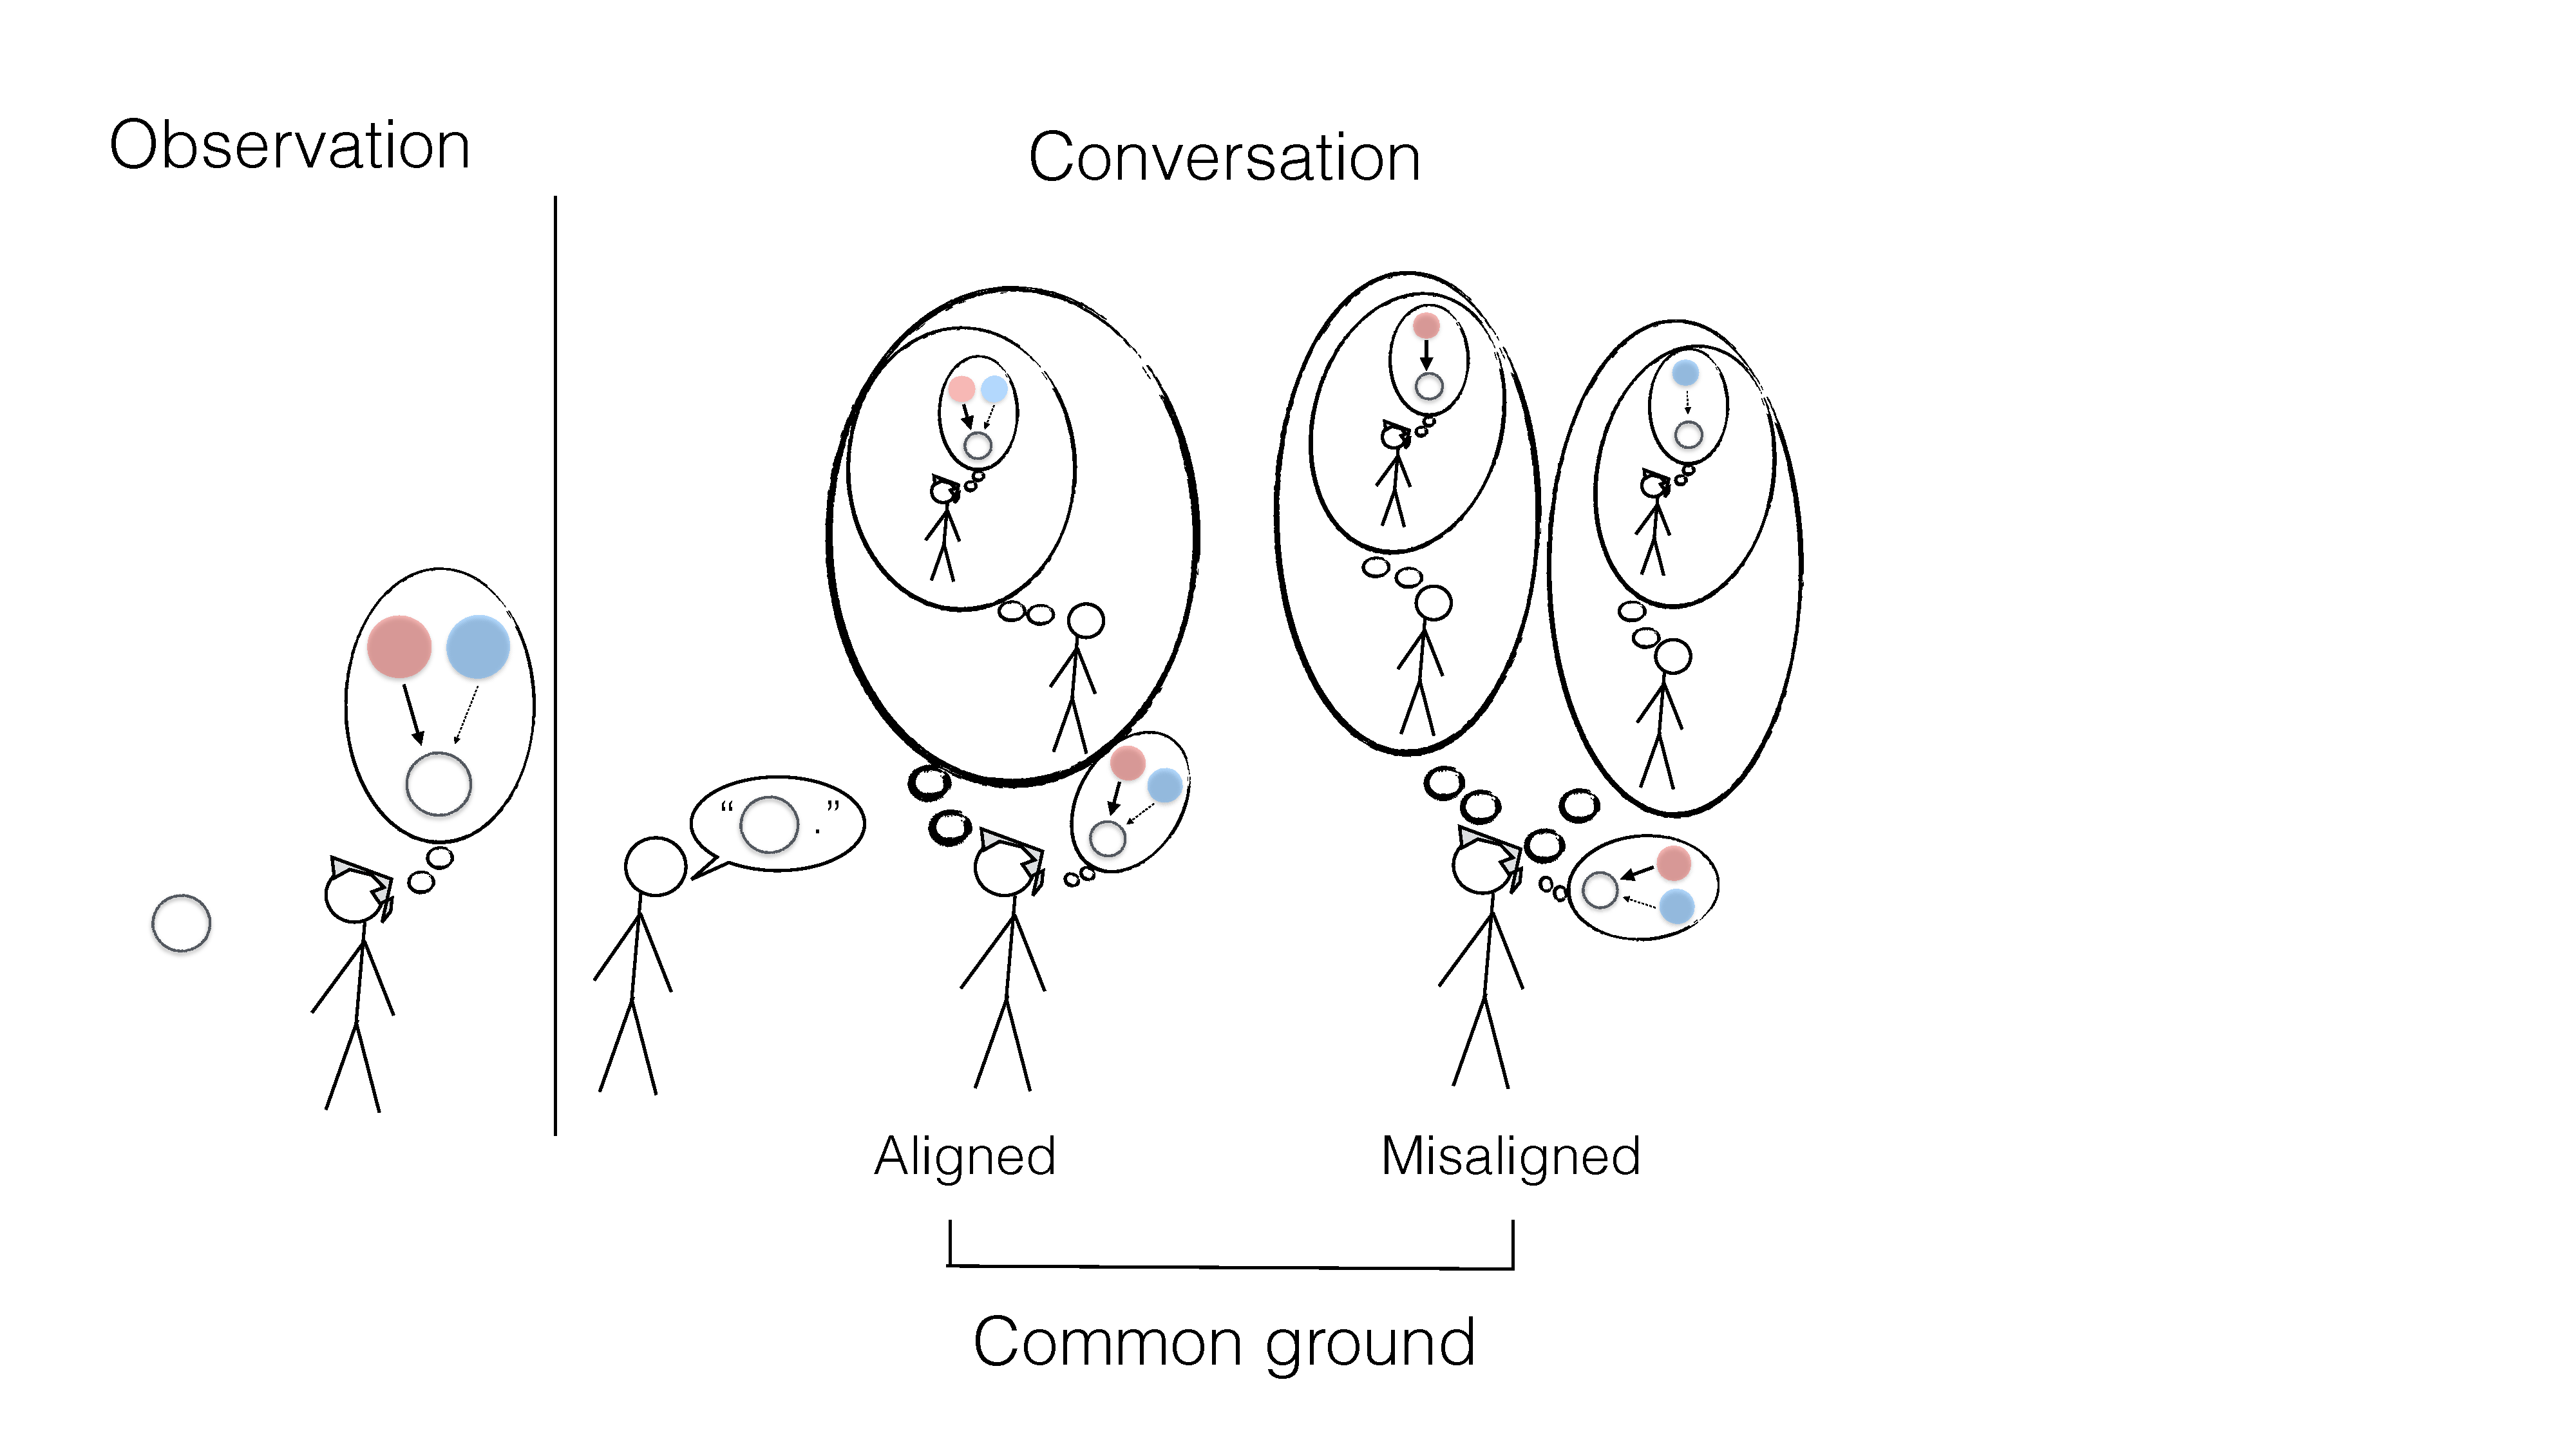
\includegraphics[width=\columnwidth]{cartoon-2}
    \caption{
        \small
How does a learner interpret evidence of an event, when she is uncertain about what could have given rise to the event (a reliable cause [red] or an unreliable cause [blue])? 
%  If a listener has uncertainty about what has given rise to an event (a reliable cause [red] or an unreliable cause [blue]), observing the event is relatively more evidence for the reliable cause (red).
%In a communicative context, a speaker who asserts that the event occurred will lead the speaker to believe the reliable cause (red) was responsible, if the listener believes the speaker is represented her uncertainty correctly (Aligned).
   Observing the event occur is relatively more evidence for the reliable cause [red]. 
    In communication, hearing about an event provides the same evidence when the listener believes the speaker represents her uncertainty accurately (Aligned common ground).
   If, instead, the listener believes the speaker is presupposing some information, the listener will be led to believe the unreliable cause [blue] gave rise to the event, as that is a more informative utterance (Misaligned).
%    When speaker and listener have common ground that is not aligned, the speaker will be interpreted as presupposing one of the possible causes, and could provide evidence for a cause that would \emph{not} reliably given rise to the event (blue).
    }
  \label{fig:cartoon}
\end{figure}
%, and communicative principles (i.e., that speakers will provide truthful, relevant, and informative information) strengthen the inferences one can draw from speech acts \cite{Grice1975}.  <--DO WE NEED THIS?
%\red{DOES THIS SEEM RIGHT?}

Critically, communication is only successful when a speaker and listener share common ground \cite{Clark1996}.
Although interlocutors often directly manage information that is in common ground by  expressing lack of understanding or asking clarifying questions, they can also use the conversational principle that utterances should be both relevant and informative \cite{Grice1975} to infer the knowledge that a speaker is presupposing in a given utterance.
For example, for a speaker to assert \emph{It was Percival who piqued the professor}, the speaker must already believe the listener to know that \emph{somebody} had piqued the professor \cite{Clark1977}.  But if the listener actually lacks this knowledge, the exchange does not fall apart; instead, the listener can accommodate the utterance by adjusting the common ground between herself and the speaker, inferring that it must be commonly known that someone had piqued the professor (von Fintel?).

\ndg{it would probably be useful to introduce the idea of \emph{accommodation}...}

Inferences about what is in common ground can have surprising ramifications.
A number of studies suggest that utterances which are \emph{a priori} redundant with one's beliefs about the world can lead listeners to search for ways to make those utterances informative \cite{Yandell1979, Wegner1981, Gruenfeld1992, Kravtchenko2015, Degen2015}.  
This can even undermine the utterance's literal meaning.  
\citeA{Wegner1981}, for example, demonstrated that newspaper headlines such as ``Bob Talbert is not linked to the Mafia'' \red{[check]} cause adults to have a more negative impression of Mr. Talbert than they would otherwise, despite denying incriminating information.  
\citeA{Gruenfeld1992} showed that uninformative newspaper headlines can actually cause people to believe the exact opposite of what those headlines claim.  
After reading the headline ``Robert Kennedy was not planning the assassination of Fidel Castro'', for example, adults in their study more strongly believed that Robert Kennedy \emph{was} planning to assassinate Fidel Castro.
Finally, \citeA{Kravtchenko2015} also recently showed that if a speaker says, ``John paid the cashier!'' as part of a story about John's trip to a grocery store, adults infer that John does not typically pay the cashier.  
All of these inferences are based on the fact that the utterance conveys redundant, or semantically uninformative, information.
In order to make the speech-act informative, listeners are wont to revise common ground, calling into question the behavior or habit that would otherwise ``go without saying''.


%that paying cashiers is a standard part of buying groceries, and can easily be inferred without the speaker having to state it explicitly (Bower et al., etc.).  Thus, in an attempt to make the utterance informative, adults assume that paying cashiers must be uncharacteristic of John.  Critically, if the story begins by asserting that John is usually broke, then adults do not make this inference, because the idea of John paying the cashier is no longer redundant with their expectations.



%Here, since the default assumption is that people are not typically linked to the mafia, this headline is not immediately informative.  
%As a result, adults construct a context that \emph{would} make the headline informative, namely, one in which Bob is known to be a bad person.  
%which denies a proposition that adults \emph{a priori} should not believe,
%
%%This is a kind of learning, analogous to learning about categories: Observing an instance of a category with a feature can be generalized  
%
%\section{Introduction}
%
%In one of the most infamous moments in U.S. presidential history, Richard Nixon declared to the press corps, "I am not a crook"€ (CITE).  On the surface, this claim argues for Nixon's innocence, as it literally states that he is not a crook.  As several researchers have shown, however, this statement contains a number of pragmatic implications that actually counter its literal, semantic meaning (CITE).  Nixon'€™s claim, for instance, presupposes that others believed that he was a crook; otherwise, it would not have been an informative statement to make, since most people presumably are not crooks (Grice, 1975).  Thus, if a listener is not aware of the Watergate scandal, or if they have no reason to question Nixon's moral status, they might actually learn from this claim that Nixon was likely corrupt in some way.
%
%\red{not shortening this yet because i think it's better to just write everything out, and then cut in the end of need be.}
%
%To date, this inferential process, or "€Å%“backfiring"€ linguistic effect, has received little attention in the literature.  In fact, most theories of language processing assert the opposite: if a person hears that Nixon is not a crook, then they should update their belief about Nixon to include this information... \red{EDIT}.  A few studies, however, provide preliminary evidence that utterances that are redundant with a listener'€™s preexisting beliefs do cause listeners to search for ways to make those utterances informative \cite{Yandell1979, Wegner1981, Gruenfeld1992, Kravtchenko2015}.  This process ultimately undermines the utterances' literal meanings.  
%%\citeA{Wegner1981}, for example, demonstrated that newspaper headlines such as "€Å%“Bob Talbert is not linked to the Mafia" [CHECK] cause adults to have a more negative impression of Bob than they would otherwise, despite not explicitly asserting any incriminating information--indeed, despite denying incriminating information.  Here, since the default assumption is that people are not typically linked to the mafia, this headline is not immediately informative.  As a result, adults construct a context that \emph{would} make the headline informative, namely, one in which Bob is known to be a bad person.  
%%\citeA{Gruenfeld1992} went even further to show that uninformative newspaper headlines can actually cause people to believe the exact opposite of what those headlines claim.  After reading the headline "€Å%“Robert Kennedy was not planning the assassination of Fidel Castro"€, for example, which denies a proposition that adults \emph{a priori} should not believe, adults in their study more strongly believed that Robert Kennedy \emph{was} planning to assassinate Fidel Castro.
%



%\red{I WOULD MOVE THE FIGURE TO THE MODEL SECTION}

%Affirming redundant information can have a similar effect \cite{Gruenfeld1992, Kravtchenko2015}.  
The phenomenon of ``backfiring utterances'' (i.e., utterances that decrease listeners' beliefs in a proposition by dint of asserting it) is vexing when paired alongside the incredible human capacity to learn from examples and testimony. 
Why is it that a speaker asserting a claim can be taken both as evidence for that claim and against that claim, depending on the situation? 
We suggest this inference depends on what is in common ground in the communicative context, and formalize the backfiring inference in a probabilistic model of language understanding.
%Figure \ref{fig:cartoon} is a sketch of the framework.
We show that the same \ndg{same?} framework predicts the backfiring effect as a function of the common ground between speaker and listener.
We empirically verify the model's predictions in a behavioral experiment designed to draw out the conditions under which this inference does and does not occur. 
Our materials also allow us to verify some of the quantitative aspects of the model---how the \emph{a priori} belief strength relates to the inference strength.
These findings have ramifications for how deliver public messages (e.g. for motivational purposes) when common ground with a reader is hard to be certain of. 

%\red{Do we want to give away all our findings upfront?  Much better intro!}
%\mht{I think so, to both Qs.}

%To our knowledge, no current model of language processing can account for this pragmatic inference.  
%$%We propose such a model in the present study.  In Experiment 1, we replicate previous findings that adults try to avoid redundancy in conversation by revising their beliefs about the world so that potentially uninformative utterances become informative \cite{Kravtchenko2015} (also cite Jaeger studies etc.).  Specifically, we ask whether utterances such as, "My student turned in her homework on time today,"€ imply that the student does not typically turn in her homework on time, despite serving as evidence for this behavior.  We then test whether our proposed model predicts these results.  We also test an important, previously unexplored(?) prediction of our model: that this "€œbackfiring"€ effect of language should be eliminated 1) when the listener makes explicit her uncertainty, for instance, about whether the student turned in his homework on time, since this would make the speaker's utterance semantically informative; and 2) when the utterance is removed from any conversational context, since this pragmatic inference depends on the \emph{conversational} agreement that utterances should be informative.



\section{Formalizing backfiring language}

Observing an event happen multiple times can be evidence for an underlying cause that could reliably give rise to the event.
Indeed, observing just one instance of an event is relatively stronger evidence for a reliable cause than an unreliable cause, all else being equal.
Similarly, observing a behavior $b$ in a person can be taken as evidence for an underlying habit $h$. 
Seeing your friend's roommate doing her dishes, for example, provides some evidence that the roommate usually does her dishes. 
It is a more likely explanation than the alternative.
%For example, if you are waiting for a bus that ends up being 15 minutes late, it is reasonable to fear it may be late the next day; public transit in this town may be unreliable. 
%disembark in a novel location to find it raining, it is reasonable to fear it may be raining in five minutes. 
%Raining events are correlated with future raining events, and this place might well be a rainy place. 

We can formalize this using a simple Bayesian model:
\begin{eqnarray}
P(h \mid b) \propto P(b \mid h) P(h) \label{eq:bayes}
\end{eqnarray}
As a habit is more likely to give rise to the behavior --- as $P(b \mid h)$ gets large --- so too does the behavior become more indicative of the habit, assuming the prior probabilities are constant. 

\ndg{this paragraph is kind of confusing and doesn't really lead into the formal treatment. revise to emphasize (and show) how to model the three situations in the experiment.}
In a conversational setting, knowledge of a person's habits may or may not be in common ground, and the speaker and listener may or may not be aware of this \cite{Clark1977, Clark1996}. 
For example, in pedagogical situations, it is valid to assume the knowledge of the habit to be communicated is \emph{not} in common ground, but that both teacher and learner have a meta-agreement on this.
Friends may also have a mutually-understood common ground about a third person; one that an overhearer might not have. 
%This same situation occurs when one of the friends assumes a bit of knowledge that the other person doesn't have (e.g. because she forgot).
%Other communicative settings may exist, where the both levels of knowledge are not in common ground. 
If a listener believes that the speaker is not representing her uncertainty correctly (e.g., because the listener has forgotten this bit of information or because the listener is overhearing a conversation), she can use the speech-act to help resolve what the speaker believes to be in common ground. 
\red{we might still want a concrete example here, but can add it later}

This can be readily incorporated into Rational Speech-Acts framework \cite{Frank2012, Goodman2013}:, as a lifted variable inference akin to the treatment by \citeA{Degen2015} and discussed in detail in \citeA{GoodmanLassiter}.
%
\begin{eqnarray}
&&P_{L_1}(b, h \mid u)\propto P_{S_1}(u \mid b, h)\cdot P(b \mid h) \cdot P(h) \label{eq:L1}\\
&&P_{S_1}(u \mid b, h) \propto \mathrm{exp}({\lambda \ln P_{L_0}(b \mid u, h))} \label{eq:S1}\\
&&P_{L_0}(b \mid u, h)\propto \denote{u}(b) \cdot P(b \mid h) \label{eq:L0}
\end{eqnarray}
%
We assume the set of utterances are remarks about the behavior occurring or not --- $b$ or $\neg b$--- as well as the possibility of not remarking on the situation, a \emph{null} utterance that has no information content.  

The prior probability of a behavior depends on the habits of the person. For simplicity, we assume that the if the habit $h$ is present, the behavior has a high probability of occurring; if the habit is absent, the probability is lower. 
\begin{eqnarray}
P(b \mid h) = \begin{cases}
0.99  & \text{if } h\\
0.5  & \text{if not } h
\end{cases} \label{eq:hab}
\end{eqnarray}

The model is implemented in the probabilistic programming language WebPPL \cite{dippl}, and a simple version can be seen at \mht{add forest page}.

\begin{figure}
\centering
    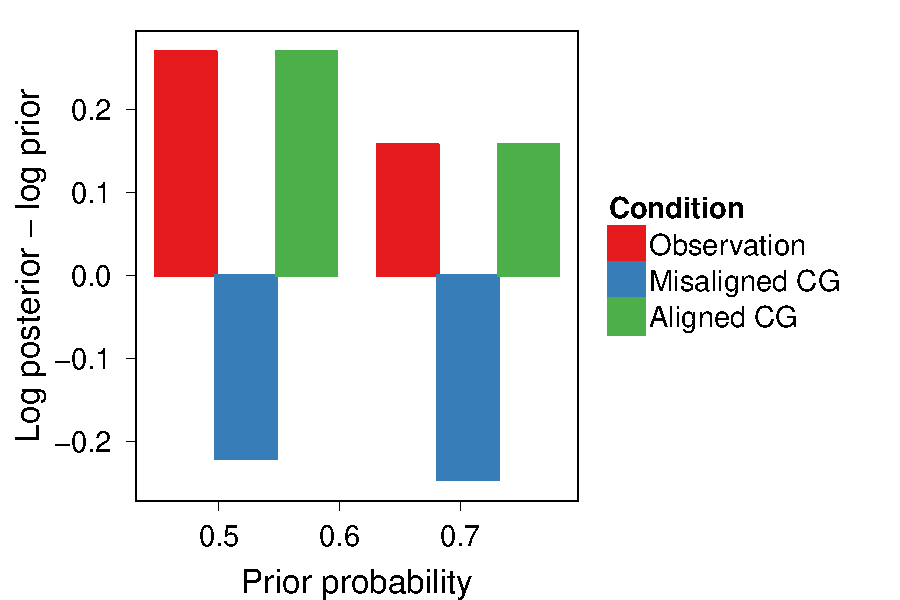
\includegraphics[width=\columnwidth]{schematic-model}
    \caption{Schematic model predictions.
    \mht{Figure made with data from posterior predictive... make figure with schematic prior data to paint the picture more visibly.}
    Observing or hearing a proposition when speaker and listener share common ground provides evidence for the underlying habit (green and red bars $> 0$). 
    When common ground is misaligned, hearing a proposition provides evidence \emph{against} the underlying habit (blue bars $<0$).
    Additionally, when the prior beliefs about a habit are least informed (prior probability around 0.5), a single observation of the behavior carries a lot of evidence, relative to when prior beliefs are more informed. 
    The opposite is true when words backfire: The stronger the \emph{a priori} belief in the habit, the more the utterance conveys evidence against that habit. }
  \label{fig:schematic-model}
\end{figure}


The model predicts that utterances affirming an event (e.g. ``My roommate washed her dishes today'') will be interpreted as expressing atypical behavior (e.g. the roommate does not typically wash her dishes) and result in a decrease in belief that the roommate has the habit of washing her dishes (Figure \ref{fig:schematic-model}).
This occurs when speaker and listener do not share common ground, but the speaker believes they do.
The strength of this inference is predicted to be modulated the listener's \emph{a priori} belief in the habit; the stronger the listener believes it to be the case that the roommate usually washes her dishes, the more the utterance \emph{My roommate washed her dishes today} will backfire. 

\subsection{Alternative models}

The backfiring inference depends critically on a misalignment of common ground. 
If a listener explicitly asks about the event occurring (e.g. ``Did your roommate wash her dishes today?''), the speaker no longer needs to be presuppose that the listener knows about the habit to make the utterance informative. 
Figure \ref{fig:schematic-model} (green bars) shows what happens when the speaker and listener have aligned common ground.
This is more akin to pedagogical communication, where teacher and learner are on the same page. 
The corresponding RSA model is:
\begin{eqnarray}
&&P_{L_1}(b, h \mid u)\propto P_{S_1}(u \mid b)\cdot P(b \mid h) \cdot P(h) \label{eq:L1mod}\\
&&P_{S_1}(u \mid b) \propto \mathrm{exp}({\lambda \ln P_{L_0}(b, h \mid u))} \label{eq:S1mod}\\
&&P_{L_0}(b, h \mid u)\propto \denote{u}(b) \cdot P(b \mid h) \label{eq:L0mod}
\end{eqnarray}
\mht{Is this right?}

Another situation where we wouldn't expect evidence to backfire is in observational learning.
Here, we would expect observing the roommate doing her dishes to be taken as evidence that she usually does her dishes. 
These predictions are borne out in a standard model of Bayesian learning (Eq.~\ref{eq:bayes}, Figure \ref{fig:schematic-model}, red bars).

\ndg{does the model predict a differences between observation and pedagogy? (it should.) cite shafto, goodman, frank for this. indicate more clearly the difference between the istructive context and the misaligned CG one... indicate why and when the listener has to accommodate by adjusting prior beliefs in order to make a statement cooperative.}

%This captures the interesting issue in communicative situations wherein if an event often occurs, then----assuming the listener and speaker both have this knowledge in common ground---it is not informative to remark on it. 
%Thus, a speaker who deliberately remarks ``My roommate did her dishes today.'' should believe that usually her roommate does not do her dishes, and believe his listener to believe this as well. 
%A listener who does not actually know whether or not the speaker's roommate usually does her dishes will interpret the utterance as implicating that the roommate does not usually do her dishes.
%We refer to the phenomena that a speech-act about an event can provide evidence against an underlying cause that would reliable give rise to the event as \emph{backfiring}. 

%We formalize the backfiring inference as a probabilistic model of pragmatic communication where listener and speaker do not share common ground. 


\section{Experiment}

\ndg{motivate experiment more clearly in terms of the modeling, and in terms of advances over previous work...}

In this experiment, we measured adults' interpretations of utterances affirming events (e.g., \emph{My roommate did her dishes today.}) in conversational settings.  
We measured interpretations both when the speaker believes the habit is in common ground and when the listener makes explicit that this is not in common ground.
Additionally, we included a control condition where the event is observed rather than uttered. 
%We tested the qualitative predictions of the pragmatics model that backfiring:
%\begin{enumerate}
%\item should occur in communicative settings where speaker and listener do not share either types of common ground (e.g., the speaker states, "My student turned in his homework on time today," while assuming that the listener knows who her student is)
%\item should not occur in communicative settings where the higher-order uncertainty about \emph{whether the event usually} occurs is in common ground (e.g., when the listener explicitly asks the speaker if the student turned in his homework on time, and the speaker replies, "Yes, my student turned in his homework on time today"); and 
%\item should not occur in settings where the lower-order uncertainty about the particular event occurring or not that are not explicitly communicative (e.g., when the listener simply observes that the speaker's student turned in his homework on time today). \end{enumerate}
Our study includes sixteen items that have considerable variability in the \emph{a priori} believability of the habit being present. 
This lets us explore how inferences may be strengthened according to the strength of adults' \emph{a priori} beliefs.

%We predicted that in communicative contexts, adults should interpret the affirmations as expressing atypical behavior (e.g., the student does not typically turn in her homework on time).  In non-communicative contexts, on the other hand, adults should interpret the utterance as reflecting typical behavior, since in these contexts there is no conversational pressure to be informative.  Instead, according to standard Bayesian reasoning(???), the affirmation should serve as evidence that the person does tend to engage in that behavior.

%In non-communicative contexts, on the other hand, adults should interpret the utterance as reflecting typical behavior, since in these contexts there is no conversational pressure to be informative.  
%Instead, according to standard Bayesian reasoning(???), the affirmation should serve as evidence that the person does tend to engage in that behavior.

\subsection{Method}

We performed a power analysis using a pilot experiment run on a subset of items to determine that we should collect 120 participants to achieve 0.95 power. 

\subsubsection{Participants}

Participants were 120 workers from Amazon's Mechanical Turk platform. 
All had at least a 95\% work approval rating.
The task took about 5 minutes and participants were compensated \$0.60.

\subsubsection{Materials}

Four versions of sixteen contexts were created (64 items in total). 
Each of the four versions was a different within-subjects condition, corresponding to the backfiring model and the two alternative models (ignorant speaker and observation) as well as a prior or baseline measurement. 
Participants completed a series of 16 randomly drawn trials from this group of 64, which were evenly distributed across conditions and included only one version of each context (i.e., participants never saw two versions of the same context).  
Trials were presented in random order.

\subsubsection{Procedure}

On each trial, participants read about Person A who could not remember either a person or a business related to Person B, and introduced to two alternatives. 
One of the alternatives was described as ``always'' \textsc{does x}, and the other alternative as ``only occasionally \textsc{does x}. 
For example:
%\textbf{Context.} 
\begin{quote}
Molly is having a hard time remembering which student her officemate is tutoring.  
She knows it is either Tom or Jim. 
Tom, she knows, always turns in his homework on time.  
Jim, she knows, only occasionally turns in his homework on time.
\end{quote}

In the \textbf{prior} condition, no additional information was provided, and participants were asked: ``Who/what is the person/business related to Person B?'' (e.g. Who is Molly's officemate tutoring?).  Response format was a 2 alternative forced-choice, with a slider bar to rate confidence.

In the three experimental conditions (misaligned common ground, aligned common ground, and observation), participants read additional information that varied according to the condition and then answered the same question.
In the \textbf{misaligned CG} condition,  Person B (e.g., Molly's officemate) says to Person A \emph{X happened}. 
In the \textbf{aligned CG} condition, Person A makes explicit that they do not know whether \textsc{X happened} today (e.g., by asking a question from a survey), and Person B clarifies for Person A \emph{X happened}.
In the \textbf{observation} condition, Person B simply observes evidence that \emph{X happened.}.
\ndg{it would be useful to have examples of each, space permitting. otherwise it's kind of hard to follow...}


%On one trial, for example, participants read the following scenario: “”  Participants then had to decide who they thought the officemate’s student was--Tom or Jim--without any other information and rate their confidence in their decision on a sliding scale.  All trials had the same structure: a character having trouble remembering information, and then a description of two options, one of which always engages in a behavior, and one of which only occasionally engages in a behavior.
%
%Pragmatic condition. The Pragmatic condition was identical to the Baseline condition, except a brief utterance was added to the vignette after the description of the two options.  In the officemate scenario, for example, participants read, “In their office, Molly’s officemate says to her, ‘My student turned in his homework on time today.’”  We predicted that in this condition adults should be more likely to state, relative to baseline, that the officemate’s student is the one who only occasionally turns in his homework on time, since that context would make the utterance informative.
%
%Literal condition. The Literal condition was the same as the Pragmatic condition, except an observation was added after the description of the two options rather than an utterance.  In the officemate scenario, this observation was, “In their office, Molly notices some papers on her officemate's desk. Her officemate's student turned in his homework on time today.”  Here, the same content is expressed--the student turned in his homework on time today--but it is no longer part of a conversation.  Thus, adults should be somewhat biased, relative to baseline, to select the student who always turns in his homework on time, since this evidence is most consistent with that behavior.
%
%Speaker Manipulation condition.  The Speaker Manipulation condition was also the same as the Pragmatic condition, except the utterance added was no longer in a communicative context(??).  Participants read, for example, “In their office, Molly helps her officemate fill out a daily report card for her student, while her officemate files away some papers.  Molly reads out loud from the report card, ‘Did your student turn in his homework on time today?’  Her officemate replies, ‘Yes. My student turned in his homework on time today.’”  Because the sentence, “My student turned in his homework on time today,” is now a response to a question on a report card rather than a spontaneous communicative act, it does not have any pragmatic implications.  As a result, participants should again be somewhat biased to select the student who always turns in his homework on time.


\subsection{Behavioral results}


\begin{figure*}
%\centering
    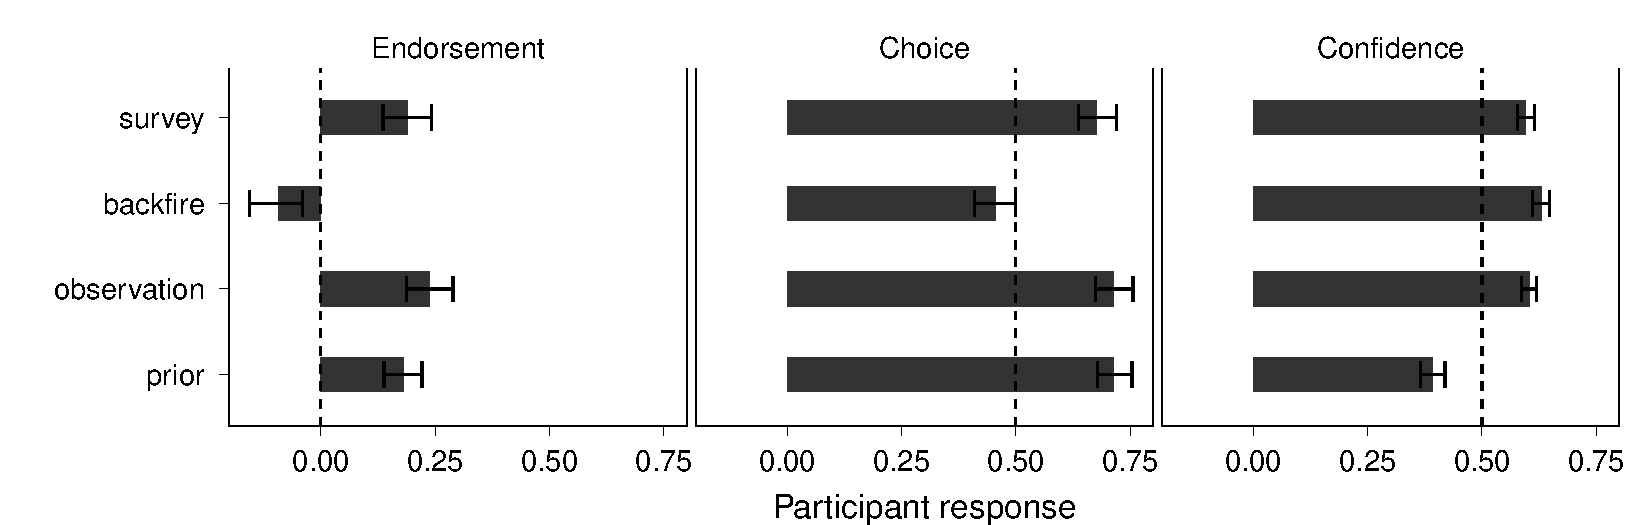
\includegraphics[width=\textwidth]{expt1-3responses}
    \caption{Dotted lines denote chance levels.}
  \label{fig:expt1-all}
\end{figure*}



We computed an \emph{endorsement score} by scaling forced-choice responses by their associated confidence level. 
We coded the selection of the more \emph{likely} response given an observation (e.g., the roommate who \emph{always} does her dishes) as a 1; the other option as -1.
We fit the \emph{endorsement score} data using a generalized mixed-effects model with random by-participant effects of intercept and random by-item effects of intercept\footnote{This was the maximal-model that our data permitted.}. 
As predicted, participants endorsed the likely response \emph{less} in the Misaligned Common Ground condition (M=-0.09; bootstrapped 95\% CI [-0.15, -0.03]) than the in the Prior condition (M=0.18 [0.14,0.22]), $\beta = -0.24; SE = 0.03; t(1794) = -8.3; p<0.001$.
There was a trend for participants to endorse the likely response \emph{slightly more} in the Observation condition (M=0.24 [0.18, 0.29]) than in the Prior condition ($\beta = 0.05; SE = 0.03; t(1794) = 1.73; p = 0.08$). 
No such trend was observed for the Aligned Common Ground condition (M=0.18 [0.13, 0.24]). 


%  condition       mean   ci_lower   ci_upper
%       (fctr)      (dbl)      (dbl)      (dbl)
%1       prior  0.1802500  0.1381531  0.2228339
%2 observation  0.2382083  0.1821380  0.2905667
%3    backfire -0.0935625 -0.1521505 -0.0345349
%4      survey  0.1887708  0.1343135  0.2415599
%Linear mixed model fit by REML 
%t-tests use  Satterthwaite approximations to degrees of freedom ['lmerMod']
%Formula: score ~ condition + (1 | workerid) + (1 | item)
%   Data: d0
%
%REML criterion at convergence: 3099.8
%
%Scaled residuals: 
%    Min      1Q  Median      3Q     Max 
%-2.5099 -0.8025  0.1406  0.7323  2.9124 
%
%Random effects:
% Groups   Name        Variance Std.Dev.
% workerid (Intercept) 0.077443 0.27829 
% item     (Intercept) 0.001255 0.03542 
% Residual             0.260483 0.51038 
%Number of obs: 1920, groups:  workerid, 120; item, 16
%
%Fixed effects:
%                       Estimate Std. Error         df t value Pr(>|t|)    
%(Intercept)           1.807e-01  3.561e-02  1.936e+02   5.075 9.04e-07 ***
%conditionobservation  5.702e-02  3.300e-02  1.796e+03   1.728   0.0842 .  
%conditionbackfire    -2.731e-01  3.299e-02  1.794e+03  -8.277 2.22e-16 ***
%conditionsurvey       6.817e-03  3.302e-02  1.797e+03   0.206   0.8364    

We further analyzed the data separately in terms of (1) the proportion of participants who selected the more \emph{likely} option given an observation (e.g. the roommate who \emph{always} does her dishes) and (2) the confidence ratings, to better understand the effect.
Critically, participants were significantly \emph{less} likely to choose the ``likely'' option in the Misaligned Common Ground condition (M=0.46 [0.41, 0.50]) than in the Prior condition (M=0.71 [0.67,0.75]) , $\beta = -1.42; SE = 0.15; p < .001$.  
Interestingly, participants were no \emph{more} likely to choose the ``likely'' option in either the observation (M=0.71 [0.68, 0.75]) or aligned CG (M=0.68 [0.63,0.71]) conditions as compared to the Prior (Figure \ref{fig:expt1-all}; middle panel).



%    condition      mean  ci_lower  ci_upper
%       (fctr)     (dbl)     (dbl)     (dbl)
%1       prior 0.3923750 0.3643260 0.4193974
%2 observation 0.6030833 0.5833073 0.6184844
%3    backfire 0.6291875 0.6102781 0.6488406
%4      survey 0.5956458 0.5757083 0.6145448

Participants are not given any helpful information in the Prior condition. 
Thus, we expected the confidence rating data to be lower in the Prior condition than in the three experimental conditions (observation, CB aligned / misaligned).
In all conditions, this was the case: Prior 0.39 [0.36, 0.42] vs. Observation 0.60 [0.58, 0.62], CG Aligned 0.60 [0.58, 0.61], CG Misaligned 0.62 [0.61, 0.64] (Figure \ref{fig:expt1-all}; right panel).

\begin{figure}
%\centering
    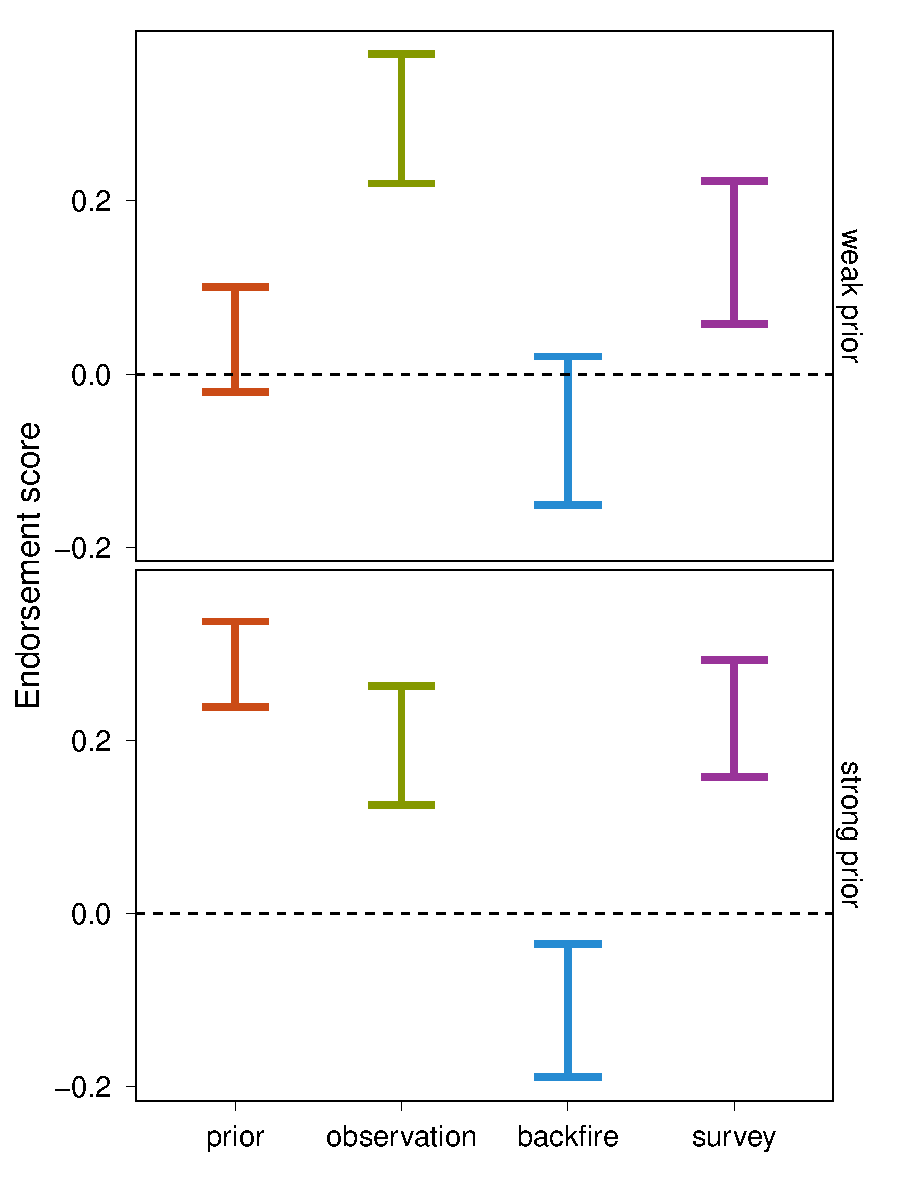
\includegraphics[width=\columnwidth]{fc2-score-medSplit}
    \caption{Median split of the data based on endorsement score in the Prior condition. 
    Dotted lines denote mean prior levels with 95\% CIs.}
  \label{fig:expt1-medspilt}
\end{figure}

The fact that we observe an effect in the CG Misaligned condition but not in the other conditions might in fact be expected if the items for which the prior beliefs are the strongest show a relatively small effect of evidence compared to when prior beliefs are the weakest.
The opposite pattern would be expected for the CG Misaligned condition, where it is predicted an utterance will backfire the most when the prior beliefs are the strongest (see Figure \ref{fig:schematic-model}) for model predictions).
To this end, we performed a median split of the items based on their prior endorsement. 
Figure \ref{fig:expt1-medspilt} shows mean endorsement score in each of the three conditions against the backdrop of the prior endorsement score, when the items are split based on prior endorsement. 
We see a larger deviation from the prior for the Observation and Aligned CG conditions and a smaller deviation from prior for the Misaligned CG condition, when the prior is relatively weak. 
The opposite pattern is observed when prior beliefs are relatively stronger, as predicted by the theory (Figure \ref{fig:schematic-model}). 

\ndg{think through the best way to analyze / present the relation to prior....}



% neither the observational data nor the utterance when common ground is aligned have an effect above and beyond the prior is not surprising \emph{if}  
%
%We were somewhat surprised to \emph{not} find an effect of the observational data or the utterance when common ground is aligned on the endorsement of the more likely response above and beyond the prior endorsement. 
%
%Reading, for example, "My student turned in his homework on time today,"€ in a communicative context caused participants to infer that the student does not typically turn in his homework on time.  
%Adults were also more confident in their choices in the Pragmatic condition (M = .63, SE = XX, n = XX) than in the Baseline condition (M = .39, SE = XX, n = XX).
%
%
%To determine how the Pragmatic, Literal, and Speaker Manipulation conditions compared to the Baseline condition, we fit the data using mixed-effects regression models comparing the responses and confidence ratings of the experimental conditions to those of the Baseline condition.  
%Each model had a fixed effect of condition and random effects of item and participant.  
%To test for the significance of effects, we performed likelihood ratio tests. 
%Chi-squared values, degrees of freedom, and p-values, all from the likelihood ratio test, are reported for each statistical test.
%
%
%The Literal (M = .71, SE = XX, n = XX) and Speaker Manipulation (M = .68,  SE = XX, n = XX) conditions, however, did not differ significantly from the Baseline condition, χ2(1) = 0, p = .98, and χ2(1) = 2.11, p = .15, respectively, even though we expected participants in these conditions to be more likely to choose the "likely"€ option.  One possibility is that for the items in this task, there was not much room for preference for the "likely"€ option to strengthen, given that participants already preferred the "likely"€ option in the Baseline condition at above-chance levels, t(119) = 9.05, p < .001.  Confidence ratings, however, did distinguish among these conditions.  Confidence ratings in both conditions (M = .60, SE = XX, n = XX in the Literal condition; M = .60, SE = XX, n = XX in the Speaker Manipulation condition) were significantly higher than confidence ratings in the Baseline condition,  χ2(1) = 275.41, p <.001, and χ2(1) = 255.68, p < .001, respectively.  Thus, the evidence provided in these two experimental conditions made adults at least more confident in their choices.  
%
%POST-HOC ANALYSES?
%To determine how pre-existing biases might influence participants'€™ responses in each of our conditions, we performed a median split analysis, separating items in the Baseline condition for which participants had weak preferences (M  = XXXX) from those for which participants had strong preferences (M = XXXX).  


\subsection{Quantitative model evaluation}

The formal pragmatics model in Eq.~\ref{eq:L1} describes how a listener is likely to interpret an utterance affirming an event, when she believes the speaker to have presupposed some information. 
Since there is appreciable variability in participants' ratings in the Prior condition, we can use those ratings as $P(h)$ and explore the quantitative predictive power of the model.
We assume, for simplicity, that the various habits described in the experimental context give rise to their associated behaviors --- $P(b \mid h)$ --- as given in Eq.~\ref{eq:hab}.
We model the Observation data using Eq.~\ref{eq:bayes}, the Misaligned CG data using Eq.~\ref{eq:L1} and the Aligned CG data using Eq.~\ref{eq:L1mod}.

The model has one remaining parameter: the speaker optimality parameter in Eqs.~\ref{eq:S1} and \ref{eq:S1mod}. 
We assume these two parameters are the same in this analysis, and infer its credible value using Bayesian data analytic techniques \cite{LW2014}. 
The posterior predictive distribution marginalizes over the likely parameter values to produce predictions about what the data should look like given the pragmatics model and the observed data. 
This is akin to fitting the parameters and is an important step in model validation as it shows what data is actually predicted by the model.
We compare the posterior predictive distribution over the probabilities of producing the \emph{likely} response to the empirical means for each item and condition (Figure \ref{fig:scatter}). 
The model provides a reasonable quantitative fit to the empirical data ($r(48) = 0.82$), though the fit is far from perfect.

One issue is that there is not an a lot of reliable variability in the human judgments within the different conditions, most notably in the Misaligned CG condition. 
We also seem to be doing the worst job capturing the data from the Observation condition using Eq.~\ref{eq:bayes}. 
This may be an artifact of the task: In order to present observational data to the participant, we used extended vignettes to explain how the protagonist was able to notice the event occur. 
Such an elaborate cover story may have raised the question to the participants of why the experimenter to choosing to supply this information. 
This may inadvertently have led to a \emph{backfiring} effect for some of the items.

\ndg{is it possible to get a wider range of predicted values from the (unaligned) model? if so, it would be worth running the corresponding experiment....}

\begin{figure}
    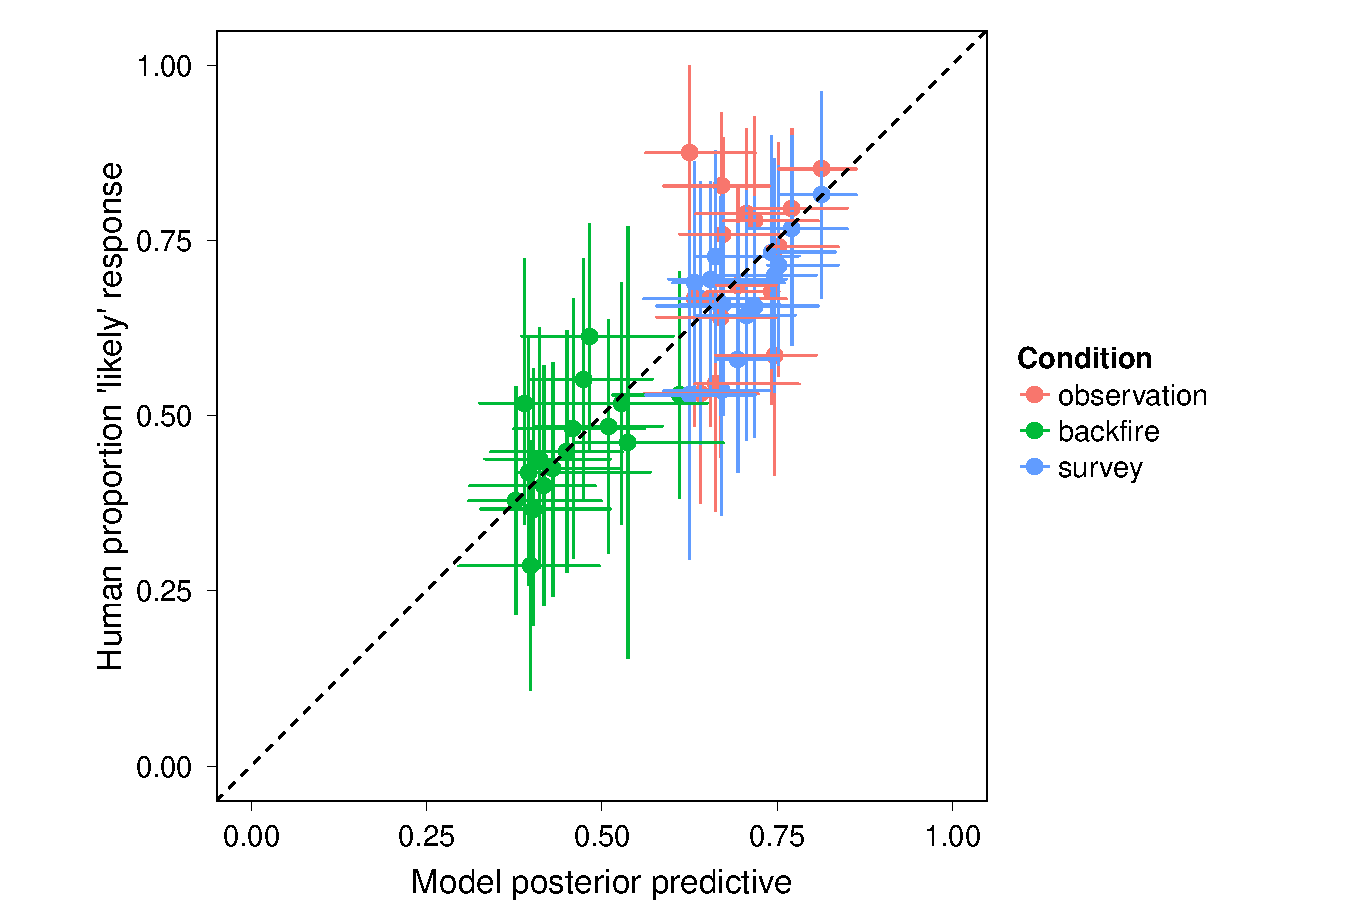
\includegraphics[width=\columnwidth]{scatter}
    \caption{Model predictions and the associated human endorsements.}
  \label{fig:scatter}
\end{figure}


%\section{Experiment 2} 
%Experiment 1 demonstrated the existence of a backfiring effect as a speech-act of what would usually be construed of as positive evidence: the observation of an event. 
%In Experiment 2, we explore downstream consequences of this inference. 
%If intuitive, structured theories of world are what guide inference, then we would expect to observe the effects of backfiring in different components of that structured konwledge.
%For example, If habits have a causal dependence on some more abstract trait, then having one's belief shaken in a person's habit can have belief shaken in the upstream trait. 
%For instance, upon hearing one's friend say \emph{My roommate did her dishes today.}, a hearer could plausibly infer both this an irregular event and that the roommate is the kind of person who wouldn't normally do her dishes. 
%That is, the roommate's room might also be a mess, she might be an inconsiderate person, or maybe more likely than not to fall delinquent on her rent checks.

%This opens the door for manifestly different types of conceptual learning from language. \red{This is a good point, but I feel like we'll end up focusing *not* on language (and instead on the relation between irregular events and traits)... which maybe is ok, I don't know.}


%and conceptually replicates \citeA{Kravtchenko2015} 


\section{Discussion}

We have presented a formal model for Common Ground inference that uses communicative principles (\emph{be truthful}, \emph{be informative}) to infer what presuppositions the speaker must have brought to conversation. 
The model predicts that an utterance that should ``go without saying'' given one Common Ground will lead a listener to infer a different Common Ground, and result in a backfiring effect decreasing the listener's belief in the proposition being affirmed.
The quantitative model predicts that this effect should be strongest when the \emph{a priori} beliefs in the common ground that would make the utterance uninformative are the strongest.
This is in contrast to typical Bayesian updating, where the most information is gained when \emph{a priori} beliefs are most uncertain. 
We validate all of these predictions in our experiment.

%We replicate previous findings that adults revise their beliefs about information that is in common ground between interlocutors so that utterances are not redundant with the preexisting beliefs of the listener (CITE).  This revision of beliefs ultimately undermines the literal content of the utterance.  Upon hearing, "My student turned in his homework on time today," for instance, adults will learn that the student turned in his homework on time, but they will also infer that the student must not \emph{typically} turn in his homework on time.

Our experiment serves as a conceptual replication of \citeA{Kravtchenko2015}.
Our work expands upon theirs in the following ways: 
(1) We include control conditions that show how the information is interpreted when it is an observation as well as when it is an utterance when common ground is aligned between speaker and listener; 
(2) We show how the strength of the inference depends systematically on the strength of the prior;
(3) We include a formal pragmatics model that predicts all of the above.

%we developed a computational model that predicts this behavior; 2) we demonstrated that adults do \emph{not} make this inference when the listener's uncertainty about the event is in common ground with the speaker, or when the utterance is removed from a conversational context (i.e., when it is framed as an observation); and 3) we provide evidence that the strength of the backfiring effect systematically varies according to the strength adults' preexisting beliefs. \red{add more explanation here}

In addition to contributing to our knowledge of language understanding, this work has practical relevance.  
Recent efforts to persuade the general public that there is no causal relation between vaccines and autism, for example, include articles titled, "Vaccines do not cause autism" \red{(cite e.g., CDC)}.  
Similarly, websites, media outlets, and researchers tend to state, ``Girls can do math,'' as a way of promoting gender equality \red{(cite e.g., Smithsonian Mag}).  
While these two statements would certainly be useful and informative for those who hold the belief that vaccines \emph{do} cause autism or that girls \emph{cannot} do math, it is unclear how they might be received by people who already share these beliefs, or who are not aware of either of these debates.  
The headline, ``Girls can do math'', for instance, could potentially signal to a naive readers that many people believe that girls cannot do math, and that there are legitimate reasons to hold this belief (e.g., perhaps girls tend to be less intelligent than boys).  
As a result, these readers might walk away doubting girls' ability to do math more than they would have otherwise.

In the present study, our focus was on affirmations of past events (e.g., ``My student turned in his homework on time''; ``The gym had clean towels today''), as a first step towards modeling this backfiring effect of language.  
Further work is necessary to determine how other kinds of affirmations, such as generic claims, might also backfire.



\bibliographystyle{apacite}

\setlength{\bibleftmargin}{.125in}
\setlength{\bibindent}{-\bibleftmargin}

\bibliography{backfiring-cogsci2016}


\end{document}
